\documentclass[12pt]{beamer}

\usepackage[english]{babel}
\usepackage[utf8]{inputenc}
\usepackage[T1]{fontenc}
\usepackage{lmodern}
\usepackage[export]{adjustbox}

\usetheme{Berlin}
\usecolortheme{spruce}

\title{how do we know how far things are}
\author{Ethan Snyder}
\date{8/12/2025}

\begin{document}
\setbeamertemplate{headline}{}

\begin{frame}
    \titlepage
\end{frame}

\section{Introduction}

    \begin{frame}
        \centering
        \large how do we know how far things are?\\
        \vspace{2em}
        \normalsize this will be our leading question\\
        \vspace{2em}
        enjoy :)
    \end{frame}
    \begin{frame}
        \centering
        parallax, mostly
    \end{frame}
    \subsection{Parallax --- Moving \& Stationary}
        \begin{frame}{parallax} \centering
            this may be what you're picturing :)
            \begin{figure}
                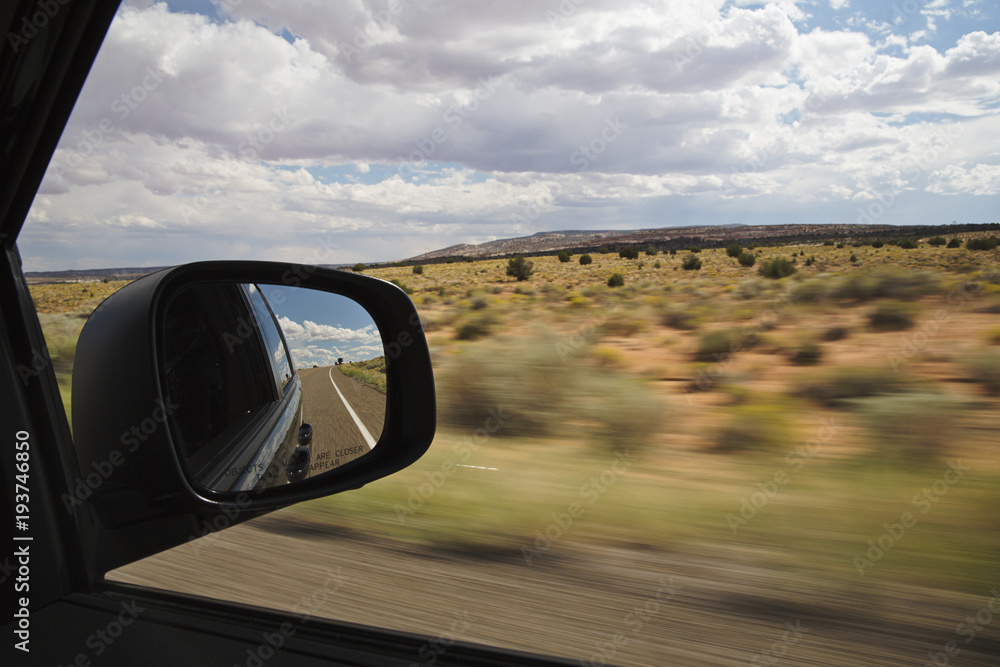
\includegraphics[scale=0.8, fbox, bb=0 0 240 160]{parallaxcar.jpeg}
                \caption{Parallax as seen looking out a moving car's window$^0$.}
            \end{figure}
            \footnotetext{\tiny Image: https://stock.adobe.com/images/view-out-the-car-window-as-the-scenery-blurs-by/193746850}
        \end{frame}
        \begin{frame}{parallax} \centering
            two types of parallax
            \pause
            \begin{columns}
                \begin{column}{0.5\linewidth}
                    \begin{block}{moving parallax}
                        \begin{itemize}
                            \item<3-> involves movement
                            \item<4-> things close to observer appear to move more, things farther appear to move less
                        \end{itemize}
                    \end{block}
                \end{column}
                \begin{column}{0.5\linewidth}
                    \begin{block}{stationary parallax}
                        \begin{itemize}
                            \item<3-> does not
                            \item<4-> the change in an objects appearance from two different locations (at once or at different times)
                        \end{itemize}
                    \end{block}
                \end{column}
            \end{columns}
            \pause[5] \vspace{1em}
            (these are actually the same, kinda. motion is just being in two places at different times :) )
        \end{frame}
        \begin{frame}{moving parallax} \centering
            moving parallax car picture again here look
            \begin{figure}
                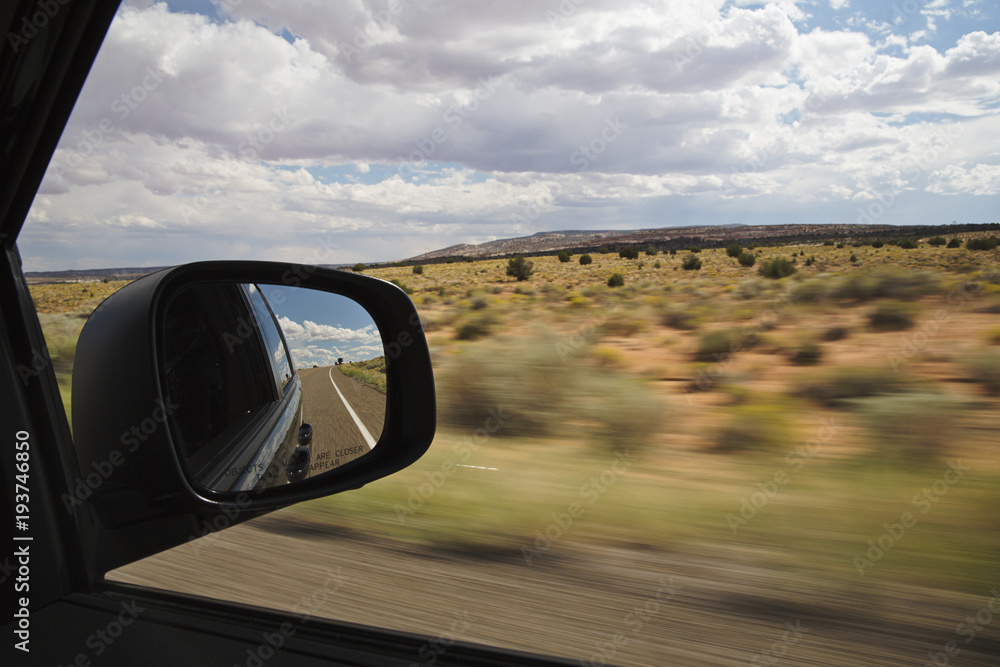
\includegraphics[scale=0.8, fbox, bb=0 0 240 160]{parallaxcar.jpeg}
                \caption{Parallax as seen looking out a moving car's window again$^0$.}
            \end{figure}
            \footnotetext{\tiny Image: https://stock.adobe.com/images/view-out-the-car-window-as-the-scenery-blurs-by/193746850}
        \end{frame}
        \begin{frame}{stationary parallax} \centering
            like human eyes, for example\\
            this is how depth perception works
            \begin{figure}
                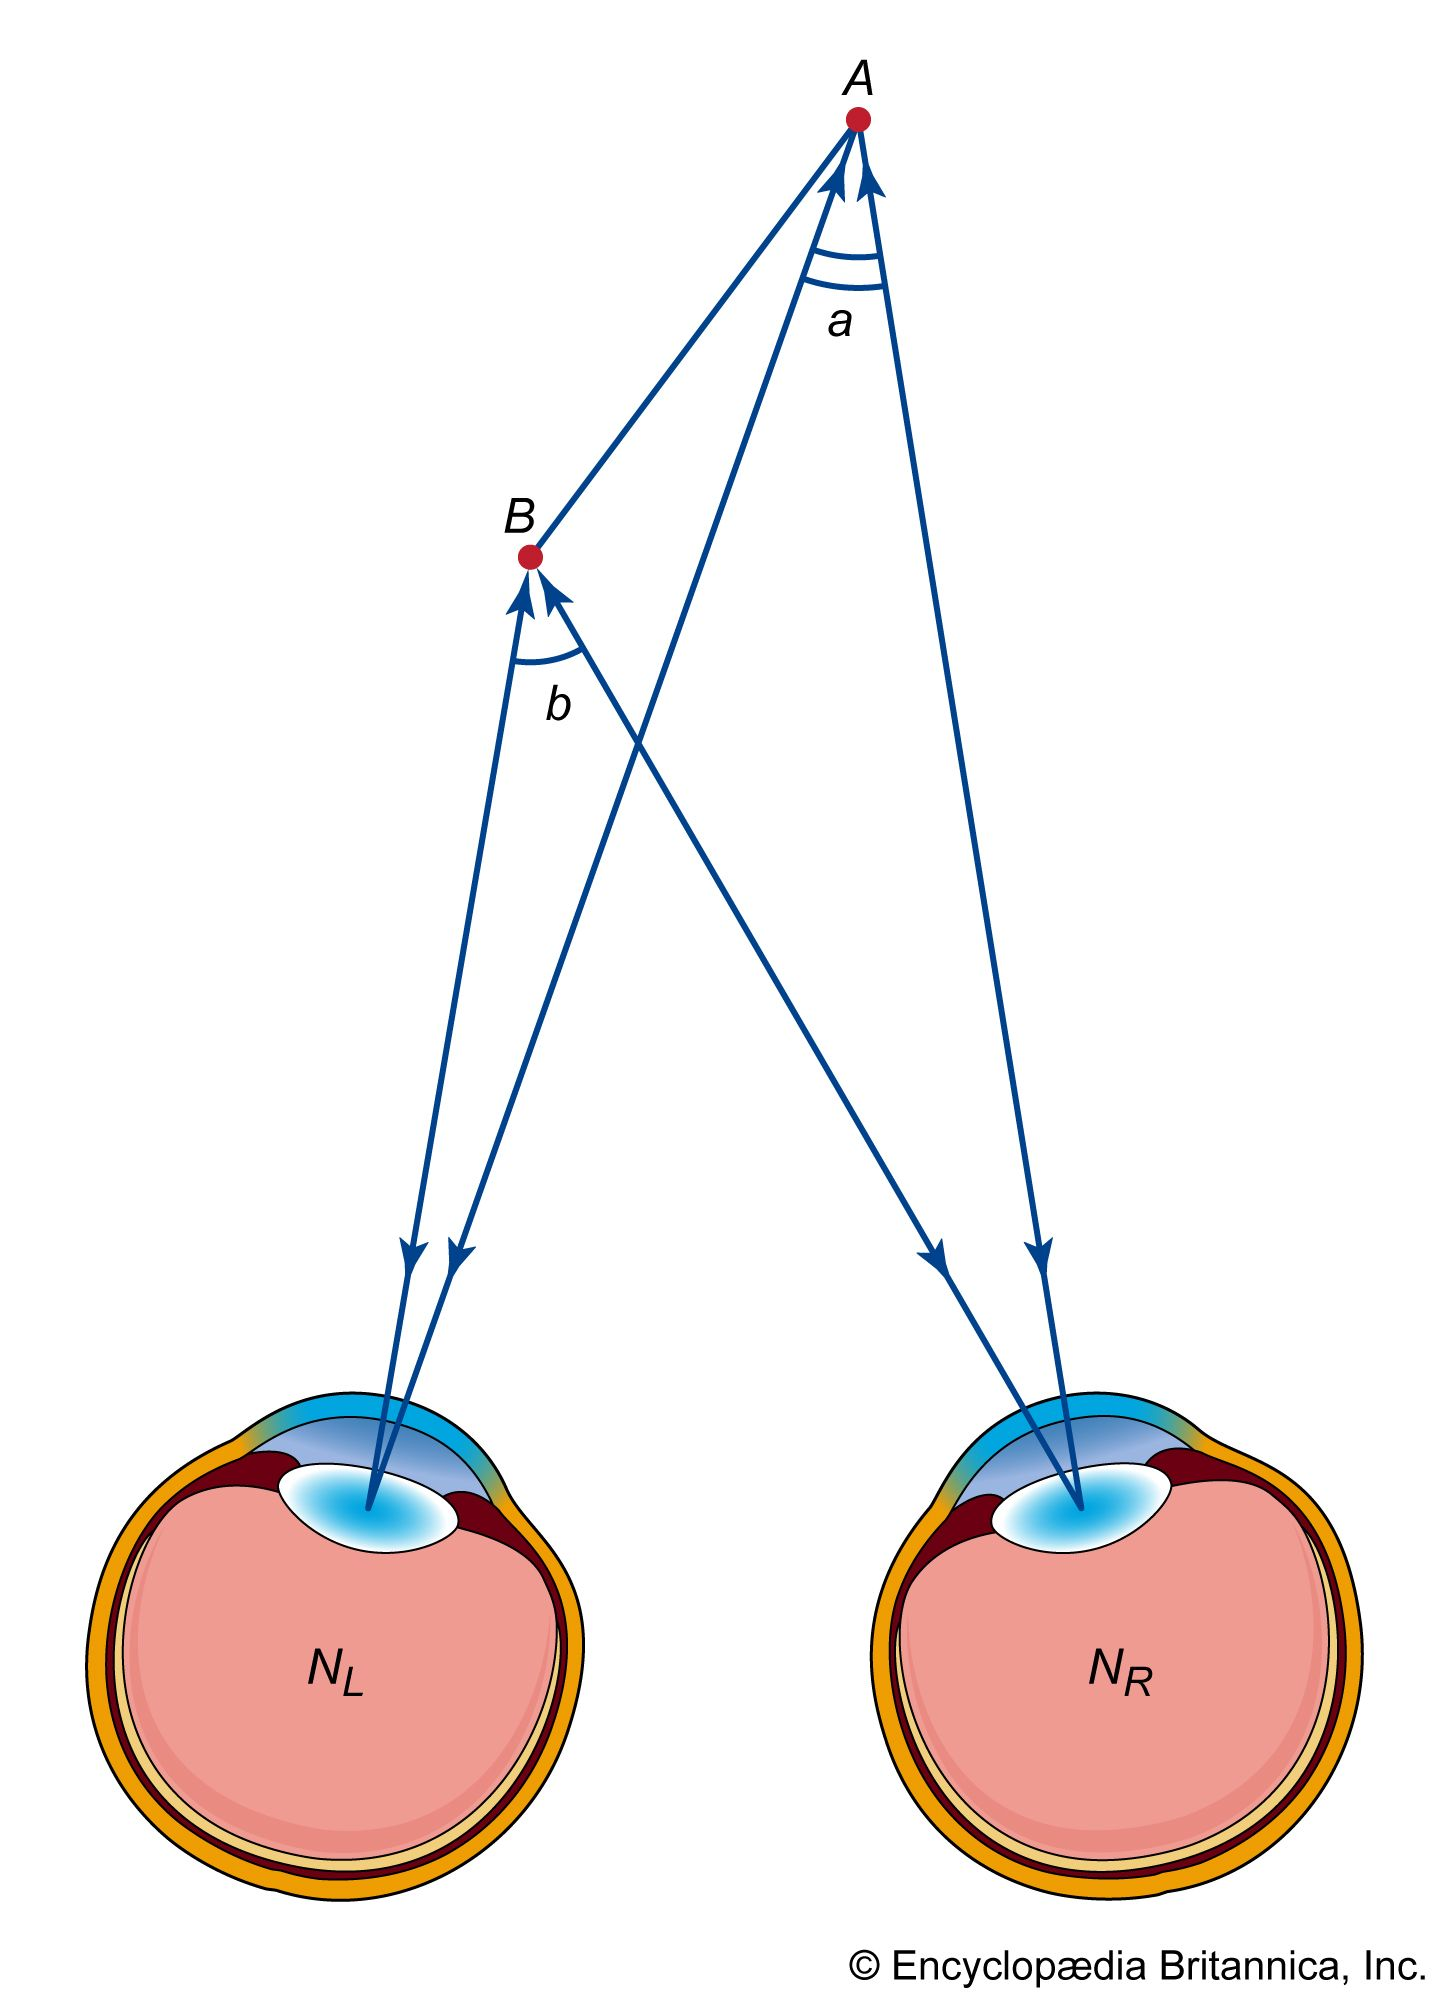
\includegraphics[scale=0.06, bb=0 0 1400 2000, fbox]{parallaxeyes.jpg}
                \caption{Eyes doing parallax$^0$.}
            \end{figure}
            \footnotetext{\tiny Image: https://cdn.britannica.com/85/4085-050-5575ACA3/parallax-points-NL-eyes-NR-left.jpg}
        \end{frame}
        \begin{frame}{summary} \centering
            we know how far things are away from us\\because we have EYES dipshit
        \end{frame}
        \begin{frame} \centering
            ok but what about numbers\\
            \vspace{2em}
            like what if we want to MEASURE a distance
        \end{frame}
        \begin{frame}
            \tableofcontents
        \end{frame}
\section{Measuring Shortish Distances}
    \subsection{Apparent Size, Units, Measuring Devices}
        \begin{frame}{Apparent Size}{What if you \textit{know the size of a distant object?}} \centering
            Easiest solution for measuring a distance.
            \begin{figure}
                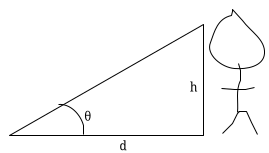
\includegraphics[scale=0.6, bb=0 0 280 160]{angletriangle.png}
            \end{figure}
            \pause
            \[\sin{\theta}=\frac{h}{d} \implies d=\frac{h}{\sin{\theta}}\]
            \pause
            (you just need to know the size of the distant object and be able to measure the angle $\theta$)
        \end{frame}

\end{document}